\documentclass[a4paper,12pt]{book}
\usepackage{mathptmx}
\usepackage{hyperref}
\usepackage{cancel}
\usepackage{amsmath}
\usepackage{amssymb}
\usepackage{graphicx}
\author{Gábor Hadházy and Tamás Hadházy}
\title{Mathematics}
\date{\today}

\begin{document}
\maketitle

\tableofcontents

% Chapter 1 - Algebra
\chapter{Algebra and Pre-calculus}
The first chapter is about algebra. It will cover the topics that was written by Gábor Hadházy and Tamás Hadházy. Algebra and Pre-calculus are the foundation of mathematics. It is important to understand the concepts of algebra and pre-calculus before moving on to more advanced topics.

\section{Essentials}
This section will cover the essentials in order to get started. 
\subsection{The set of Real numbers}
\begin{itemize}
    \item $\mathbb{N} = \{1, 2, 3, ...\}$ - - The set of natural numbers. 
    \item $\mathbb{Z} = \{..., -2, -1, 0, 1, 2, ...\}$ - The set of integers.
    \item $\mathbb{Q} = \{\frac{a}{b} | a, b \in \mathbb{Z}, b \neq 0\}$ - The set of rational numbers. 
    \item $\mathbb{I}$ - The set of Irrational Numbers(Real numbers that are not rational). 
    \item $\mathbb{R} = \mathbb{Q} \cup \mathbb{I}$
\end{itemize}


\subsection{The properties of Real numbers}
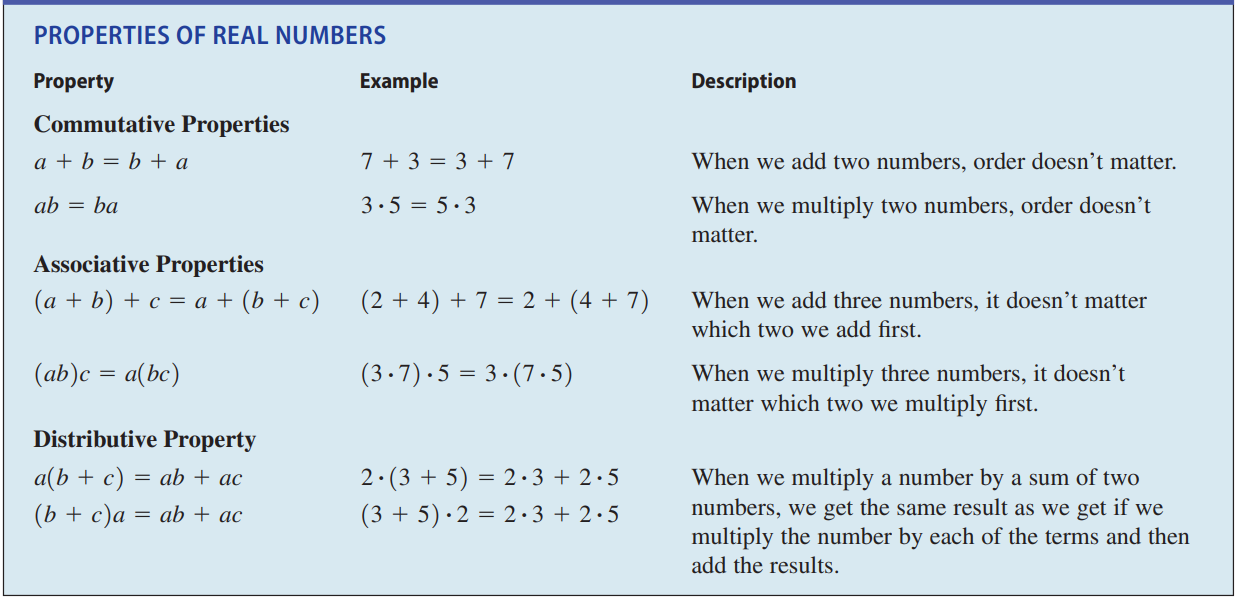
\includegraphics[width=1.1\textwidth]{algebra-pre-calculus/essentials/properties.png}

\subsection{Addition and Subtraction}
The number 0 is special for addition; it is called the additive identity because $a+0=a$ for any real number $a$. Every real number $a$ has a negative, $-a$, that satisfies $a+(-a)=0$. Subtraction is the operation that undoes addition; to subtract a number from another, we simply add the negative of that number. By definition
$$
a-b=a+(-b)
$$
To combine real numbers involving negatives, we use the following properties.
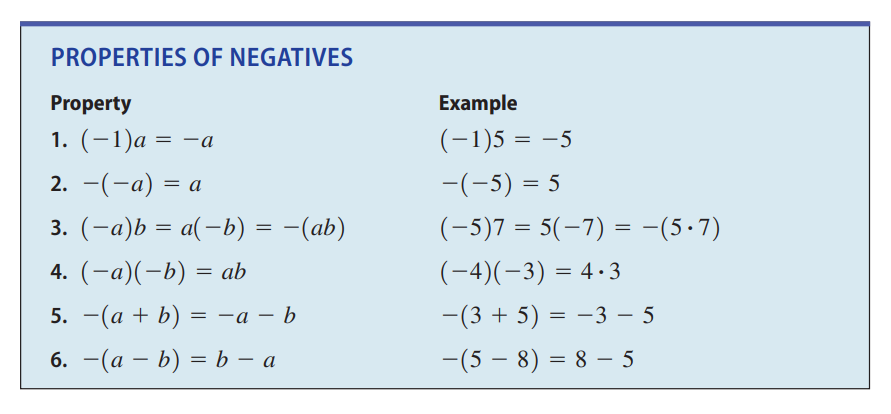
\includegraphics[width=1.1\textwidth]{algebra-pre-calculus/essentials/properties_addition_subtraction.png}

Property 6 states the intuitive fact that $a-b$ and $b-a$ are negatives of each other. \\
Property 5 is often used with more than two terms:
$$
    -(a+b+c)=-a-b-c
$$

\subsection{Multiplication and Division}
The number 1 is special for multiplication; it is called the \textbf{multiplicative identity} because $a \cdot 1=a$ for any real number $a$. Every nonzero real number $a$ has an inverse, $1 / a$, that satisfies $a \cdot(1 / a)=1$. Division is the operation that undoes multiplication; to divide by a number, we multiply by the inverse of that number. If $b \neq 0$, then, by definition,
$$
a \div b=a \cdot \frac{1}{b}
$$
We write $a \cdot(1 / b)$ as simply $a / b$. We refer to $a / b$ as the quotient of $a$ and $b$ or as the fraction $a$ over $b$; $a$ is the numerator and $b$ is the denominator (or divisor). To combine real numbers using the operation of division, we use the following properties. \\
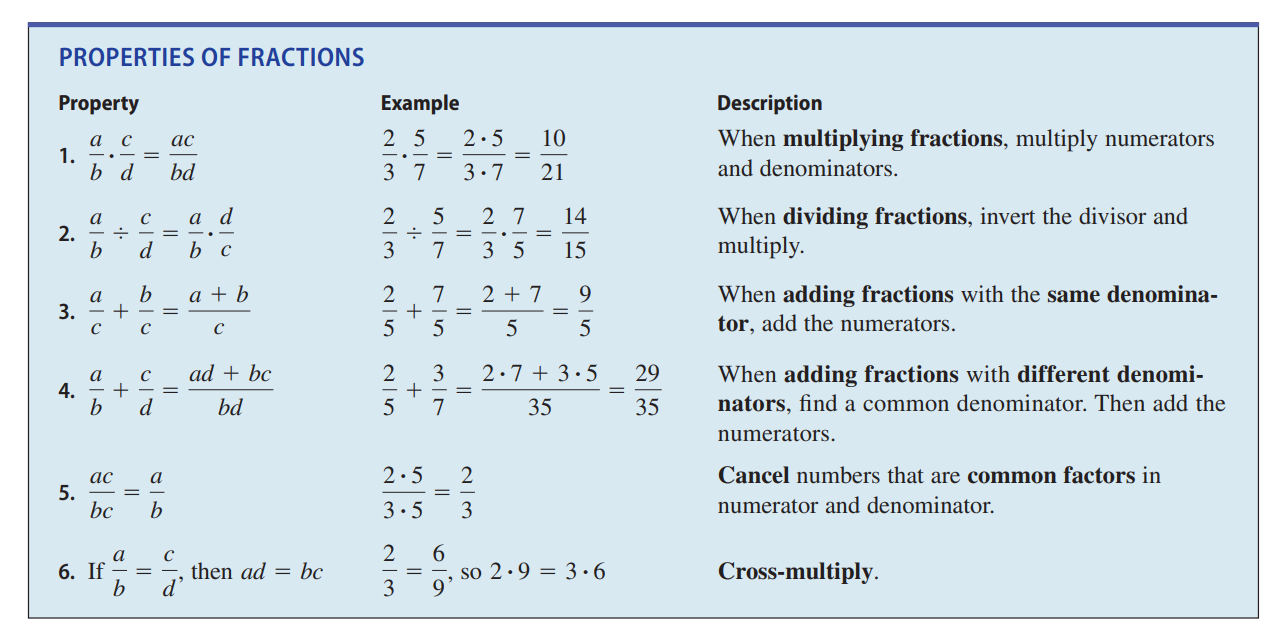
\includegraphics[width=1.1\textwidth]{algebra-pre-calculus/essentials/properties_multiplication_division.png}

When adding fractions with different denominators, we don’t usually use Property 4.
Instead we rewrite the fractions so that they have the smallest possible common denominator (often smaller than the product of the denominators), and then we use Property 3. This
denominator is the Least Common Denominator (LCD) described in the next example.

\subsection{Using the LCD to Add Fractions}

Evaluate: $\frac{5}{36}+\frac{7}{120}$
\textbf{Solution.} Factoring each denominator into prime factors gives
$$
36=2^2 \cdot 3^2 \quad \text { and } \quad 120=2^3 \cdot 3 \cdot 5
$$
We find the least common denominator (LCD) by forming the product of all the prime factors that occur in these factorizations, using the highest power of each prime factor. Thus the LCD is $2^3 \cdot 3^2 \cdot 5=360$. So
$$
\begin{aligned}
\frac{5}{36}+\frac{7}{120} & =\frac{5 \cdot 10}{36 \cdot 10}+\frac{7 \cdot 3}{120 \cdot 3} & \text { Use common denominator } \\
& =\frac{50}{360}+\frac{21}{360}=\frac{71}{360} & \begin{array}{l}
\text { Property } 3: \text { Adding fractions with the } \\
\text { same denominator }
\end{array}
\end{aligned}
$$

\subsection{Real line}

The real numbers can be represented by points on a line, as shown below. The
positive direction (toward the right) is indicated by an arrow. We choose an arbitrary
reference point O, called the origin, which corresponds to the real number 0. Given any
convenient unit of measurement, each positive number x is represented by the point on
the line a distance of x units to the right of the origin, and each negative number -x is
represented by the point x units to the left of the origin. The number associated with the
point P is called the coordinate of P, and the line is then called a coordinate line, or a
real number line, or simply a real line. Often we identify the point with its coordinate
and think of a number as being a point on the real line.

\begin{align*}
    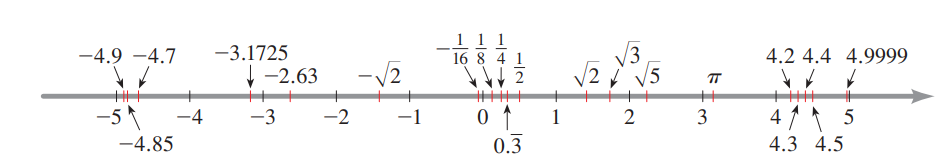
\includegraphics[width=1.1\textwidth]{algebra-pre-calculus/essentials/real-line.png}
\end{align*}

\section{Absolute Value and Distance}
The absolute value of a number $a$, denoted by $|a|$ , is the distance from $a$ to 0 on
the number line. Distance is always positive or zero, so we have
$|a|\geq0$ for every number $a$. Remembering that $-a$ is positive when $a$ is negative, we have the following definition.

\begin{equation*}
    |a| = \begin{cases}
        \;a  & \textnormal{if} \ a \geq 0 \\
        \;-a & \textnormal{if} \ a < 0
    \end{cases}
\end{equation*}

(a) $|3|=3$ \\
(b) $|-3|=-(-3)=3$ \\
(c) $|0|=0$ \\
(d) $|3-\pi|=-(3-\pi)=\pi-3 \quad($ since $3<\pi \quad \Rightarrow \quad 3-\pi<0)$

\subsection{Properties of Absolute Value}
\begin{enumerate}
    \item $|a| \geq 0$
    \item $|a|=|-a|$
    \item $|a b|=|a||b|$
    \item $\displaystyle \left|\frac{a}{b}\right|=\frac{|a|}{|b|}$
    \item $|a+b| \leq|a|+|b|$
\end{enumerate}

\subsection{Distance Between Points on the Real line}

What is the distance on the real line between the numbers -2 and 11? From
Figure 11 we see that the distance is 13. We arrive at this by finding either
$ |11-(-2)|=13$ or $|(-2)-11=13|$. From this observation we make the following definition. \\

If $a$ and $b$ are real numbers, then the \textbf{distance} between the points $a$ and $b$ on the real line is: \\
$$ d(a,b)=|a-b| $$

From the Property 6 of negatives it follows that
$$ |b-a| = |a-b|$$
$$ |3-7| = |7-3| = 4 $$

This confirms that, as we would expect, the distance from a to b is the same as the
distance from b to a.

\textbf{Example.} The distance between then numbers -8 and 2 is $d(-8,2)=|-8-2|=|-10|=10$.

\subsubsection*{Exercises}
For Exercises please download the book from here(\url{https://faculty.ksu.edu.sa/sites/default/files/precalculus-mathematics_for_calculus-j._stewart_l._redlin_and_s._watson-cengage_learning_7th_edition_2015.pdf}) and you can go to the 37th page for exercises.  % Section 1 - Essentials
\section{Exponentiation}
When starting out with Exponentiation it is important first to understand the different parts of an exponential expression, so let's consider:
$$b^x = \underbrace{b \cdot b \cdot ... \cdot b}_{x \ times}$$
\begin{itemize}
  \item $b$ is the \textbf{base}.
  \item $x$ is the \textbf{exponent}.
\end{itemize}

As a reminder $ x^0 = 1 $

Let's discuss the different rules of Exponentiation:
\subsection{Product Rule}
To find the product of two exponential expression with the same base, add the exponents. 
$$ x^{n} \cdot x^{m} = x^{n+m} $$

\subsection{Quotient Rule}
When two exponential expressions with the same base are divided,  to find their quotient subtract their exponents. 
$$ \frac{x^n}{x^m} = x^{n-m} $$

\subsection{Power Rule}
When you raise an power to a power in an exponential expression to get the product, multiply the exponents
$$ (x^{n})^{m} = x^{n \cdot m} $$ 
$$ OR $$
$$ (x^{n})^{m} = \underbrace{x^n \cdot ... \cdot x^n}_{m \ times} $$
Here it is proven that the power rule is simply just the product rule.

\subsection{Negative Exponents}
When dealing with negative exponents this equation will apply: 
$$ x^{-n} = \frac{1}{x^n} $$

Since, 
$$ \frac{1}{x} = \frac{x^0}{x^1} = x^{0-1} = x^{-1} $$
It is important to note that this is just only one way of proving this, there are a couple more. 

\subsection{Fractional Exponents}
$$ \large x^{\frac{1}{n}} = \sqrt[n]{x} $$
The proof of this can be found in the next section \hyperref[sec:radicals]{Radicals(click to redirect)}.

\subsection{Additional rules}
Distribute an exponent over a product: $(x \ y)^{n} = x^{n} \ y^{n}$ \\
Distribute an exponent over a quotient: $  (\frac{a}{b})^{n} = \frac{a^{n}}{b^{n}}$

\begin{align*}
  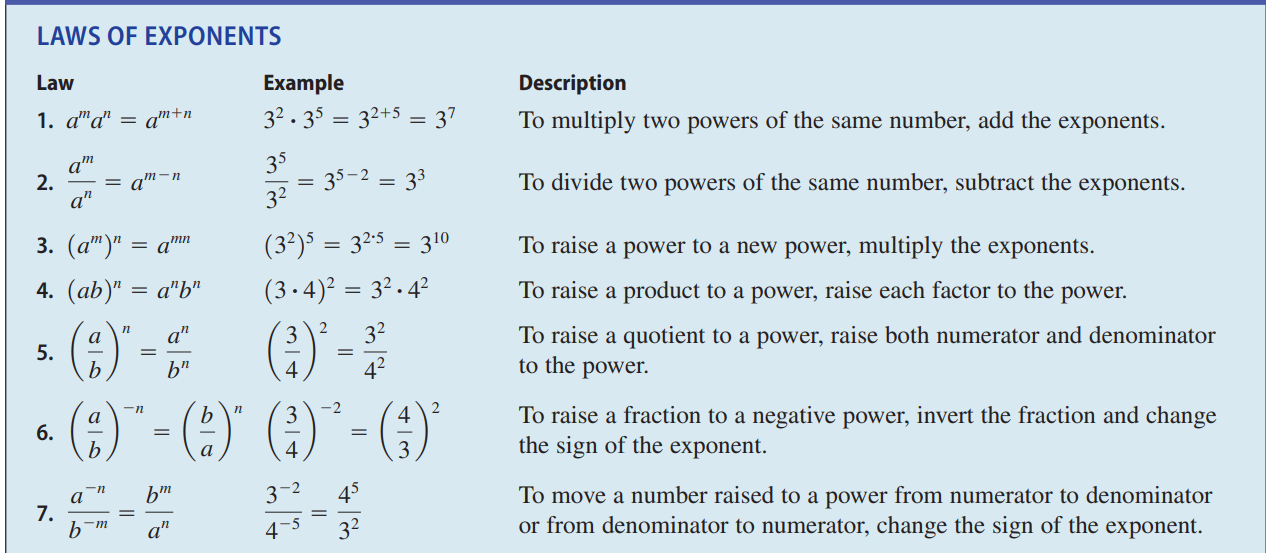
\includegraphics[width=1.2\textwidth]{algebra-pre-calculus/exponentiation/laws-of-exponents.png}
\end{align*}

\newpage % Section 2 - Exponentiation
\label{sec:radicals}
\section{Radicals}
$$ \large \sqrt[n]{x} $$
\begin{itemize}
  \item $x$ is the \textbf{radicand}.
  \item $n$ is the \textbf{index}(nth root).
  \item $\large \sqrt[n]{x}$ expression is the \textbf{radical}
\end{itemize}

As promised let's look at the fractional exponent equation. If $n$ is a positive integer that is greater than $1$ and a is a real number then,
$$ \sqrt[n]{a} = a^{\frac{1}{n}} $$

We are often referring the left side of the equation as the \textbf{radical form} and the right side of the equation as the \textbf{exponent form}

\subsubsection{Proof}
In order to prove this equation we can establish first this: 
$$ (a^{\frac{1}{n}})^{n} = a^{n \cdot \frac{1}{n}} = a^{\frac{n}{n}} = a $$
Let's take an example to avoid confusion: 
$$ (9^{\frac{1}{2}})^2 = 9^{\frac{1}{2} \cdot2} = 9^{\frac{2}{2}} = 9 $$

To put this into words $ 9^{\frac{1}{2}} $ is the number that when squared will return back $ 9 $. In other words this is exactly what it meant by the root(in this case square root) which will return back the number that when squared it will be 9. Therefore: 
$$ 9^{\frac{1}{2}} =  \sqrt[2]{9} = 3 $$

Since,
$$ (3)^2 = 9 = (9^{\frac{1}{2}})^2 $$

Therefore the equation has been proven: 
$$ \sqrt[n]{a} = a^{\frac{1}{n}} $$

It is very important to note a misconception here. The index is required in these radical expressions to make sure that we correctly evaluate the radical. There is one exception to this rule and that is square root.
$$ \sqrt[2]{a} = \sqrt[]{a} $$
In every other cases we \textbf{must} define the index, because otherwise it will be considered as a square root, Whenever working with square roots the index can be omitted.

\subsubsection{General rational exponent}
Since, $ a^{\frac{1}{n}} = \sqrt[n]{a} $.
Let's establish the general rational exponent in terms of radicals as follows. 
$$ a^{\frac{m}{n}} = (a^{\frac{1}{n}}) ^{m} = (\sqrt[n]{a})^m $$
$$ OR $$
$$ a^{\frac{m}{n}} = (a^m) ^{\frac{1}{n}} = \sqrt[n]{a^m} $$

Since being aware of the \textbf{Associative Property of Multiplication}, the order of the multiplication can be changed. 

Therefore, 
$$ a^{\frac{m}{n}} = \sqrt[n]{a^m} $$

\subsection{Properties of radicals}
\begin{itemize}
  \item $\sqrt[n]{a^n} = a$ \ This is simply true because when trying to find the $n$th root of a number and  also raising the number to that power then that's simply will be equal to the number.  \\
Consider this as an example,
$$ \sqrt[]{9^2} = \sqrt[]{81} = 9$$
   \item $ \sqrt[n]{ab} = \sqrt[n]{a} \sqrt[n]{b} $ \\
   To prove this consider this, \\
    1. Start with the left-hand side (LHS) of the equation,
    $ \sqrt[n]{ab} $ Using the definition of the nth root:
    $ \sqrt[n]{ab} = (ab)^{\frac{1}{n}} $ \\
    2. Next apply the product rule of exponents, which states that $ a^m \cdot a^n = a^{m+n} $ Therefore, $ (ab)^{\frac{1}{n}} = a^{\frac{1}{n}} \cdot b^{\frac{1}{n}} $ \\ 
    3. Now, rewrite the exponents as radicals:
    $ a^{\frac{1}{n}} $ is equivalent to $ \sqrt[n]{a} $ and $ b^{\frac{1}{n}} $ is equivalent to $ \sqrt[n]{b} $ \\
    4. So, we have: $ a^{\frac{1}{n}} \cdot b^{\frac{1}{n}} = \sqrt[n]{a} \cdot \sqrt[n]{b} $ \\
    5. Finally this proves that: $ \sqrt[n]{ab} = \sqrt[n]{a} \cdot \sqrt[n]{b} $
    \item $ \large \sqrt[n]{\frac{a}{b}} = \frac{\sqrt[n]{a}}{\sqrt[n]{b}} $ To prove this consider this, \\
    1. As previously Start with the left-hand side (LHS) of the equation: $ \sqrt[n]{\frac{a}{b}} $ \\
    2. Now using the definition of the nth root: $ \sqrt[n]{\frac{a}{b}} = \left(\frac{a}{b}\right)^{\frac{1}{n}} $ \\
    3. Apply the power rule of the exponents which states that: \\ $ (a^m)^{\frac{1}{n}} = a^{m \cdot \frac{1}{n}} = a^{\frac{m}{n}}$, Therefore when we are dealing with a fraction as the base it is the same when dealing with numbers that are not fractions: 
$$ \left(\frac{a}{b}\right)^{\frac{1}{n}} = \frac{a^{\frac{1}{n}}}{b^{\frac{1}{n}}} $$ Since, \\
$$ (\frac{a}{b})^c = \frac{a^c}{b^c} $$ \\
With an example: $ (\frac{a}{b})^2 = \frac{a}{b} \cdot \frac{a}{b} = \frac{a^2}{b^2} $ \\
	4. Now rewrite the exponents as radicals: $ a^{\frac{1}{n}} $ is equivalent to $ \sqrt[n]{a} $ and  $b^{\frac{1}{n}}$ is equivalent to $ \sqrt[n]{b} $ \\
	5. So, we have: 
	$$ \frac{a^{\frac{1}{n}}}{b^{\frac{1}{n}}} = \frac{\sqrt[n]{a}}{\sqrt[n]{b}} $$ \\
	6. Finally, this proves that: 
	$$ \sqrt[n]{\frac{a}{b}} = \frac{\sqrt[n]{a}}{\sqrt[n]{b}} $$ \\
	\\
	
	\item Also note that while we can “break up” products and quotients under a radical we can’t do the same thing for sums or differences. In other words,
	$$ \sqrt[n]{a+b} \neq \sqrt[n]{a}+ \sqrt[n]{b}  $$ 
	$$ AND $$
	$$ \sqrt[n]{a-b} \neq \sqrt[n]{a}- \sqrt[n]{b} $$ \\
These can simply be proven by examples, 
$$ 5 = \sqrt25 = \sqrt{9+16} \neq \sqrt9 + \sqrt16 = 3+4 = 7 $$

\end{itemize} % Section 3 - Radicals
\section{Factorials}
In mathematics, the factorial of a non-negative integer(whole number (not a fractional number) that can be positive, negative, or zero.) $ n $, denoted by $ n! $, is the product of all positive integers less than or equal to $ n $ \\

$$ 5! = 5 \cdot 4 \cdot 3 \cdot 2 \cdot 1 = 123 $$ \\
Generically expressing, 
$$ n! = n \cdot (n-1) \cdot (n-2) \cdot (n-3) \cdot ... \cdot 3 \cdot 2 \cdot 1 $$

\subsection{Operations with factorials}
Let's clarify a couple of easy examples, 
$$ 2! + 3! = 2 \cdot 1 + 3 \cdot 2 \cdot 1 = 8 $$ 
$$ 3! 4! = 3 \cdot 2 \cdot 1 \cdot 4 \cdot 3 \cdot 2 \cdot 1 = 144 $$ \
When it comes to a fraction of factorials there are some tricks to implement: 
$$ \frac{9!}{7!} = \frac{9 \cdot 8 \cdot 7!}{7!} = 9 \cdot 8 = 72$$
Since, $ 7! = 7 \cdot 6 \cdot 5 \cdot 4 \cdot 3 \cdot 2\cdot 1 $ \\
Consider a similar example: 
$$ \frac{4!5!}{6!} = \frac{(4 \cdot 3 \cdot 2 \cdot 1)(5!)}{6 \cdot 5!} = \frac{24}{6} = 4 $$ \\ 
Also make sure to note these rules:
$$ a! \cdot b! \neq (a + b)! $$ 

This rule applies for addition, subtraction, and division as well. 
So, 
$$ (a!)(b!) \neq (a+b)! $$
$$ \frac{(a!)}{(b!)} \neq (a-b)! $$
$$ (a!) - (b!) \neq (a-b)! $$

\subsection{Algebraic Expressions with factorial}
When dealing with different concepts it is always very important to establish generic / general equations. \\ 
For example let's consider this equation:
$$ \frac{(n+1)!}{n!} = n+1 $$ 

In order to prove this equation there can be two different approaches.
\subsubsection{Proof 1 - Easier and more genuine way of proving it}
This way is the easier way but this doesn’t prove it algebraically/mathematically it just only takes two example and assume that the general equation \textbf{must} be true. 
$$ \frac{(n+1)!}{n!} = n+1 $$
$$ \frac{8!}{7!} = \frac{8 \cdot \cancel{7!}}{\cancel{7!}} = 8 $$
This very easily proves it, however when dealing with research or more advanced mathematics this is not a valid proof. Everything has to be proved algebraically and mathematically.

\subsubsection{Proof 2 - Mathematically proven}
Before seeing the actual proof equation, let's establish a general equation for factorial.
$$ (n+1)! = (n+1) \cdot n! $$
This is true because of the definition of factorial. \\ Meaning that $ (n+1)! = (n+1) \cdot n \cdot (n-1) \cdot (n-2) \cdot ... \cdot 3 \cdot 2 \cdot 1 $ \\
Therefore, 
$$ \frac{(n+1)!}{n!} = \frac{(n+1) \cdot \cancel{n!}}{\cancel{n!}} = n+1 $$
With subtraction,
$$ \frac{(n-1)!}{n!} = \frac{\cancel{(n-1)!}}{n \cdot \cancel{(n-1)!}} = \frac{1}{n} $$

Obviously, different numbers could have been used other than $ 1 $. 
So for example,
$$ \frac{(n+2)!}{n!} = \frac{(n+2) \cdot (n+1) \cdot \cancel{(n)!} }{\cancel{n!}} = (n+2)(n+1) $$
$$ \frac{(2n + 1)!}{(2n)!}  = \frac{(2n + 1) \cdot \cancel{(2n)!}}{\cancel{(2n)!}} = 2n + 1 $$

With this in mind, working with factorials algebraically shouldn't cause any problem. 

\subsection{Other use case of factorial}
Factorial can be used in many different ways. For example in probability, it can be used for combinations. Let's say that we have four different colours and we have to choose four of them. How many different combinations can we have? 
$$ 4! = 4 \cdot 3 \cdot 2 \cdot 1 = 24$$ % Section 4 - Factorials




\section{Summations}
In mathematics, summation is the addition of a sequence of any kind of numbers, called addends or summands; the result is their sum or total. 
Let's say that we have a sequence of numbers and we want to add them up.

\subsubsection{Summation notation - Sigma notation}
$$  \sum_{i=1}^{n} a_i = a_1 + a_2 + a_3 + \ldots + a_n $$
\begin{itemize}
  \item $ i $ = index of summation
  \item $ n $ = upper limit of summation
\end{itemize}
To understand this let's consider this: 
$$ \sum_{i=1}^{4} i = 1 + 2 + 3 + 4$$
\begin{itemize}
  \item $ i = 1 $, $ i $ is the index of summation, meaning that the number where the summation starts from(in this case $ i = 1 $ so $1$).
  \item $ 4 $ is the upper limit of summation, meaning that the number where the summation ends at(in this case $ 4 $). It is important to note that the upper limit only indicates the limit for the index $i$ and doesn't indicate the number of terms that will be included in the summation.
  \item $ i $ is the formula/rule of summation. Meaning that an expression that will be used in our sequence of numbers. Quite literally the expression that will be used in the summation. This can be as complex as we would like it to be.
\end{itemize}

Let's break down the steps of the summation notation:
\begin{itemize}
  \item Firstly we start at whatever the index is, in this case it is $1$ so we start from there. 
  \item Set $i$ equal to one and then write the $1$ down. 
  \item Then we increment the index $i$, and again writing $i$ down and then summing each of these terms as we go.
  \item We continue this process until we reach the upper limit of summation, in this case it is $4$.
  \item Finally we add up all of the terms that we wrote down.
\end{itemize}

\subsubsection{Examples}
Let's consider these examples:
$$ \sum_{i = 1}^{50} \pi \cdot i^2  = \pi0^2 + \pi1^2 + \pi2^2 + \ldots + \pi(50)^2$$
$$ \sum_{i = 0}^{3} (i^2 + 2i + 4) = (0 + 0 + 4) + (1+2+4) + (4+4+4) + (9+6+4) = 42$$
$$ \sum_{i = 0}^{3} (3i + 2)^2 = 4+25+63+121 = 214$$
 % Section 5 - Summations
% Chapter 1 end - Algebra

% % Chapter 2 - Linear Algebra
% \chapter{Linear Algebra}
% The second chapter is about linear algebra. It will cover the topics that was written by Gábor Hadházy and Tamás Hadházy.
% \section{Linear Equations}

A linear equation is an equation in which the highest power of the variable is always 1. It is also known as a one-degree equation. 
Additionally A linear equation is an equation that can be written as the sum of numbers(coefficients) times variables, added up to equal to a number.

For example. $ 2x + 3y + 7.3z = 5 $ is a linear equation.

\begin{itemize}
    \item $4x^2 + 5x + 6 = 0$ is not a linear equation because the highest power of the variables is 2.
    \item $ \frac{1}{3}uv + \frac{2}{3}u = \frac{3}{5}v $ is not a linear equation because it includes a product of variables.
    \item $ 5a + 2 = 6b - \sqrt[]{2c}  $ is a linear equation because if we rearrange it, we will get: 
    $$ 5a - 6b + \sqrt[]{2c} = -2 $$
\end{itemize}

a system of linear equations (or linear system) is a collection(set) of one or more linear equations involving the same variables

For example, 
\begin{align*}
    3x + 2y - z &= 1 \\
    2x - 2y + 4z &= -2 \\
    -x + \frac{1}{2}y -z &= 0
\end{align*}
is a system of three equations in the three variables $x, y, z$. A solution to a linear system is an assignment of values to the variables such that all the equations are simultaneously satisfied. \\
A solution to the system above is given by the ordered tuple.
$$ {\displaystyle (x,y,z)=(1,-2,-2)} $$  
\subsection{Solving systems of Linear Equations with the method of substitution}
It is important to establish that there are limitless ways to solve systems of linear equations. 
Example. Solve the system of linear equations(we are going to use the method of substitution): 
\begin{align*}
    -2a + 3b + 4c = 1 \\
    a + b + 5c = 2 \\
    b = 2a + c
\end{align*}
Firstly we already have a value for $b$ in the 3rd equation so let's just substitute it into the first two equations.
\begin{align*}
    &1. \quad -2a + 3(2a + c) + 4c = 1 \\
    &2. \quad a + (2a + c) + 5c = 2 \\ 
    &3. \quad  b = 2a + c   
\end{align*}

Let's simplify the first two equations.
After expanding and simplifying the first two terms we will get:
\begin{align*}
    &1.\quad 4a + 7c = 1 \\
    &2.\quad 3a + 6c = 2 \\
    &3.\quad b = 2a + c      
\end{align*}
Notice that now we have two equations with two variables, so we can solve for $a$ and $c$.
\\ 

\begin{itemize}
    \item In the first equation we can subtract $7c$ and then divide by $4$ to get $a$. Which will give us: 
    \begin{align*}
        1. \quad  a = \frac{1}{4} - \frac{7}{4}c \\
        2. \quad 3a + 6c = 2 \\
        3. \quad b = 2a + c
    \end{align*}
    \item Now that we have the value for $a$ we can substitute that into the second equation. Which will give us:
    \begin{align*}
        &1. \quad a = \frac{1}{4} - \frac{7}{4}c \\
        &2. \quad 3(\frac{1}{4} - \frac{7}{4}c) + 6c = 2 \\
        &3. \quad b = 2a + c
    \end{align*}
    \item Now let's simplify the second equation. After expanding and simplifying with the like terms we will get:
    \begin{align*}
        &1. \quad a = \frac{1}{4} - \frac{7}{4}c \\
        &2. \quad \frac{3}{4} - \frac{21}{4}c + 6c = 2 \xrightarrow{\text{add like terms}} \frac{3}{4} + \frac{3}{4}c = 2\\
        &3. \quad b = 2a + c
    \end{align*}
    \item Now that we have this, we can simply subtract $\frac{3}{4}$ then simplify it down to: 
    $$ c = \frac{5}{3} $$ 
    \item Since we have the value for $c$ now let's figure out the value for $a$.
    $$ a = \frac{1}{4} - \frac{7}{4}(\frac{5}{3}) = \frac{1}{4} - \frac{35}{12} = - \frac{32}{12} = -\frac{8}{3}$$
    Therefore, $ a = - \frac{8}{3} $
    \item Now that we have the value for $a$ and $c$ we can substitute that into the third equation to get the \textbf{actual} value for $b$.
    $$ b = 2(-\frac{8}{3}) + \frac{5}{3} = -\frac{16}{3} + \frac{5}{3} = -\frac{11}{3}$$
\end{itemize}

Now finally we have solved the system of linear equations and we have the values for $a, b, c$. If we'd plug them in into the original equations then it would satisfy all of them. \\ 
We can list the values in an ordered tuple like this:
$$ {\displaystyle (a,b,c)=(-\frac{8}{3},-\frac{11}{3},\frac{5}{3})} $$
Now let's see another way of solving systems of linear equations.
\subsection{Solving systems of Linear Equations with the method of elimination}
Example. Solve the system of linear equations(we are going to use the method of elimination): 
\begin{align*}
    &1. \quad -2a + 3b + 4c = 1 \\
    &2. \quad a + b + 5c = 2 \\ 
    &3. \quad  b = 2a + c   
\end{align*}
Let's rearrange this system by writing each equation in the standard form, where all the variables are on the left side and the constants are on the right side.
The first two equations are already in the standard form, but the third one is not. So let's rearrange it.

\begin{align*}
    &1. \quad -2a + 3b + 4c = 1 \\
    &2. \quad a + b + 5c = 2 \\ 
    &3. \quad  -2a + b - c = 0  
\end{align*} % Section 1 - Linear Equations


\end{document}